\chapter{Project 3: LED Party}

\section{Overview}
This project adds on to the lessons from the last project. In addition to our single LED and button,
attach several more LEDs. This will let us write some code that can control them in interesting ways
and patterns. Over the course of this project, you will:
\begin{itemize}
    \item Expand the circuits from previous projects with more components
    \item Write a program that can orchestrate multiple LEDs with simple animations
    \item Respond to user input by changing the animation that is running
\end{itemize}
At the end of this project, your microcontroller should run a MicroPython program which changes the
animations that the LEDs show when the button is pushed. Let's get started!
\begin{figure}[H]
\centering
    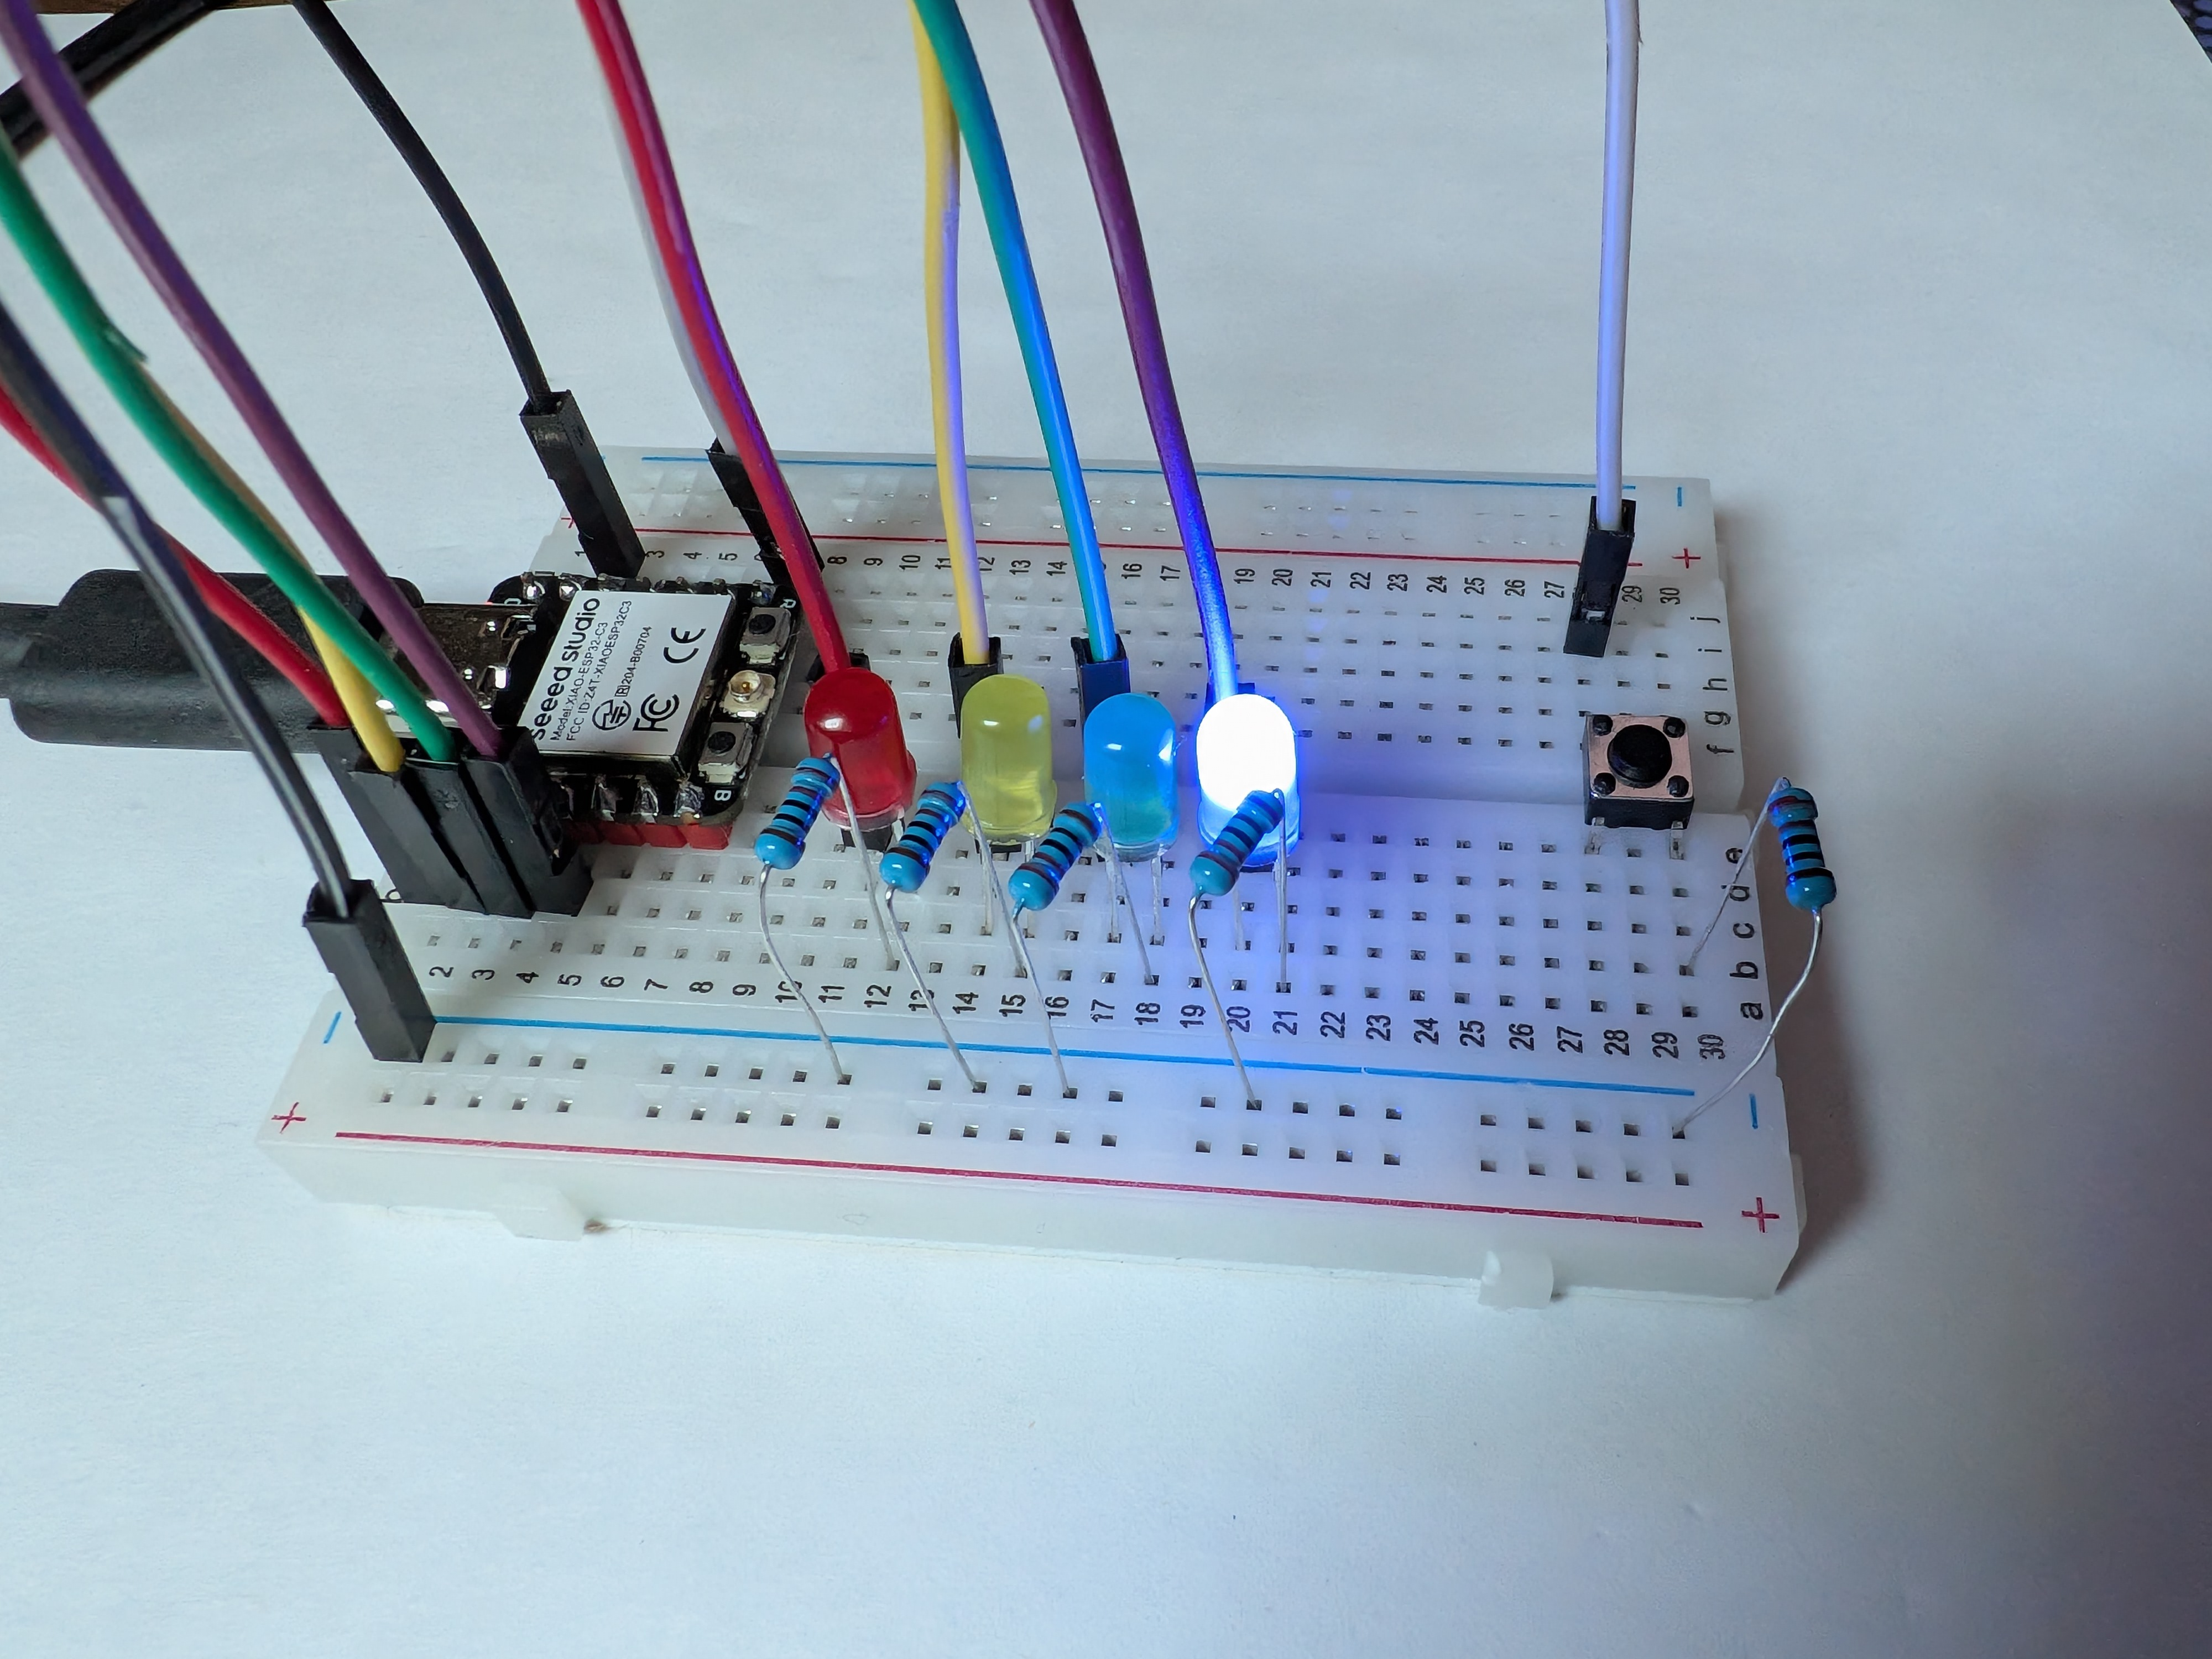
\includegraphics[width=.6\linewidth]{project_3/success!.jpg}
    \caption{The end result should look something like this}
\end{figure}

\pagebreak

\section{Directions}

\subsubsection{Remove previous components}
Before beginning, remove any components from prior chapters including LEDs, buttons, and wires. You may leave the
microcontroller attached to the breadboard.

\subsection{Creating the circuit}
Using jumper cables, you will be assembling a circuit between your microcontroller, your breadboard,
some LEDs, a pushbutton, and 220\si{\ohm} resistors for the LEDs and button.

\subsubsection{Attach the microcontroller to the breadboard}
Carefully insert the pins at the bottom of your microcontroller into the breadboard, making sure that the microcontroller is oriented such that:
\begin{itemize}
    \item The pin labeled \textbf{3V3} is inserted in hole at \textbf{Column C, Row 1} of the breadboard (or \textbf{C1}, for short)
    \item The pin labeled \textbf{Vin} is inserted in hole \textbf{J1} of the breadboard
    \item The pin labeled \textbf{D0} is inserted in hole \textbf{C15} of the breadboard
    \item the pin labeled \textbf{A0} is inserted in hole \textbf{J15} of the breadboard
\end{itemize}
You may need to apply more pressure than expected to seat the microcontroller properly in the breadboard. When its over, it should look like this:

\begin{figure}[H]
    \centering
    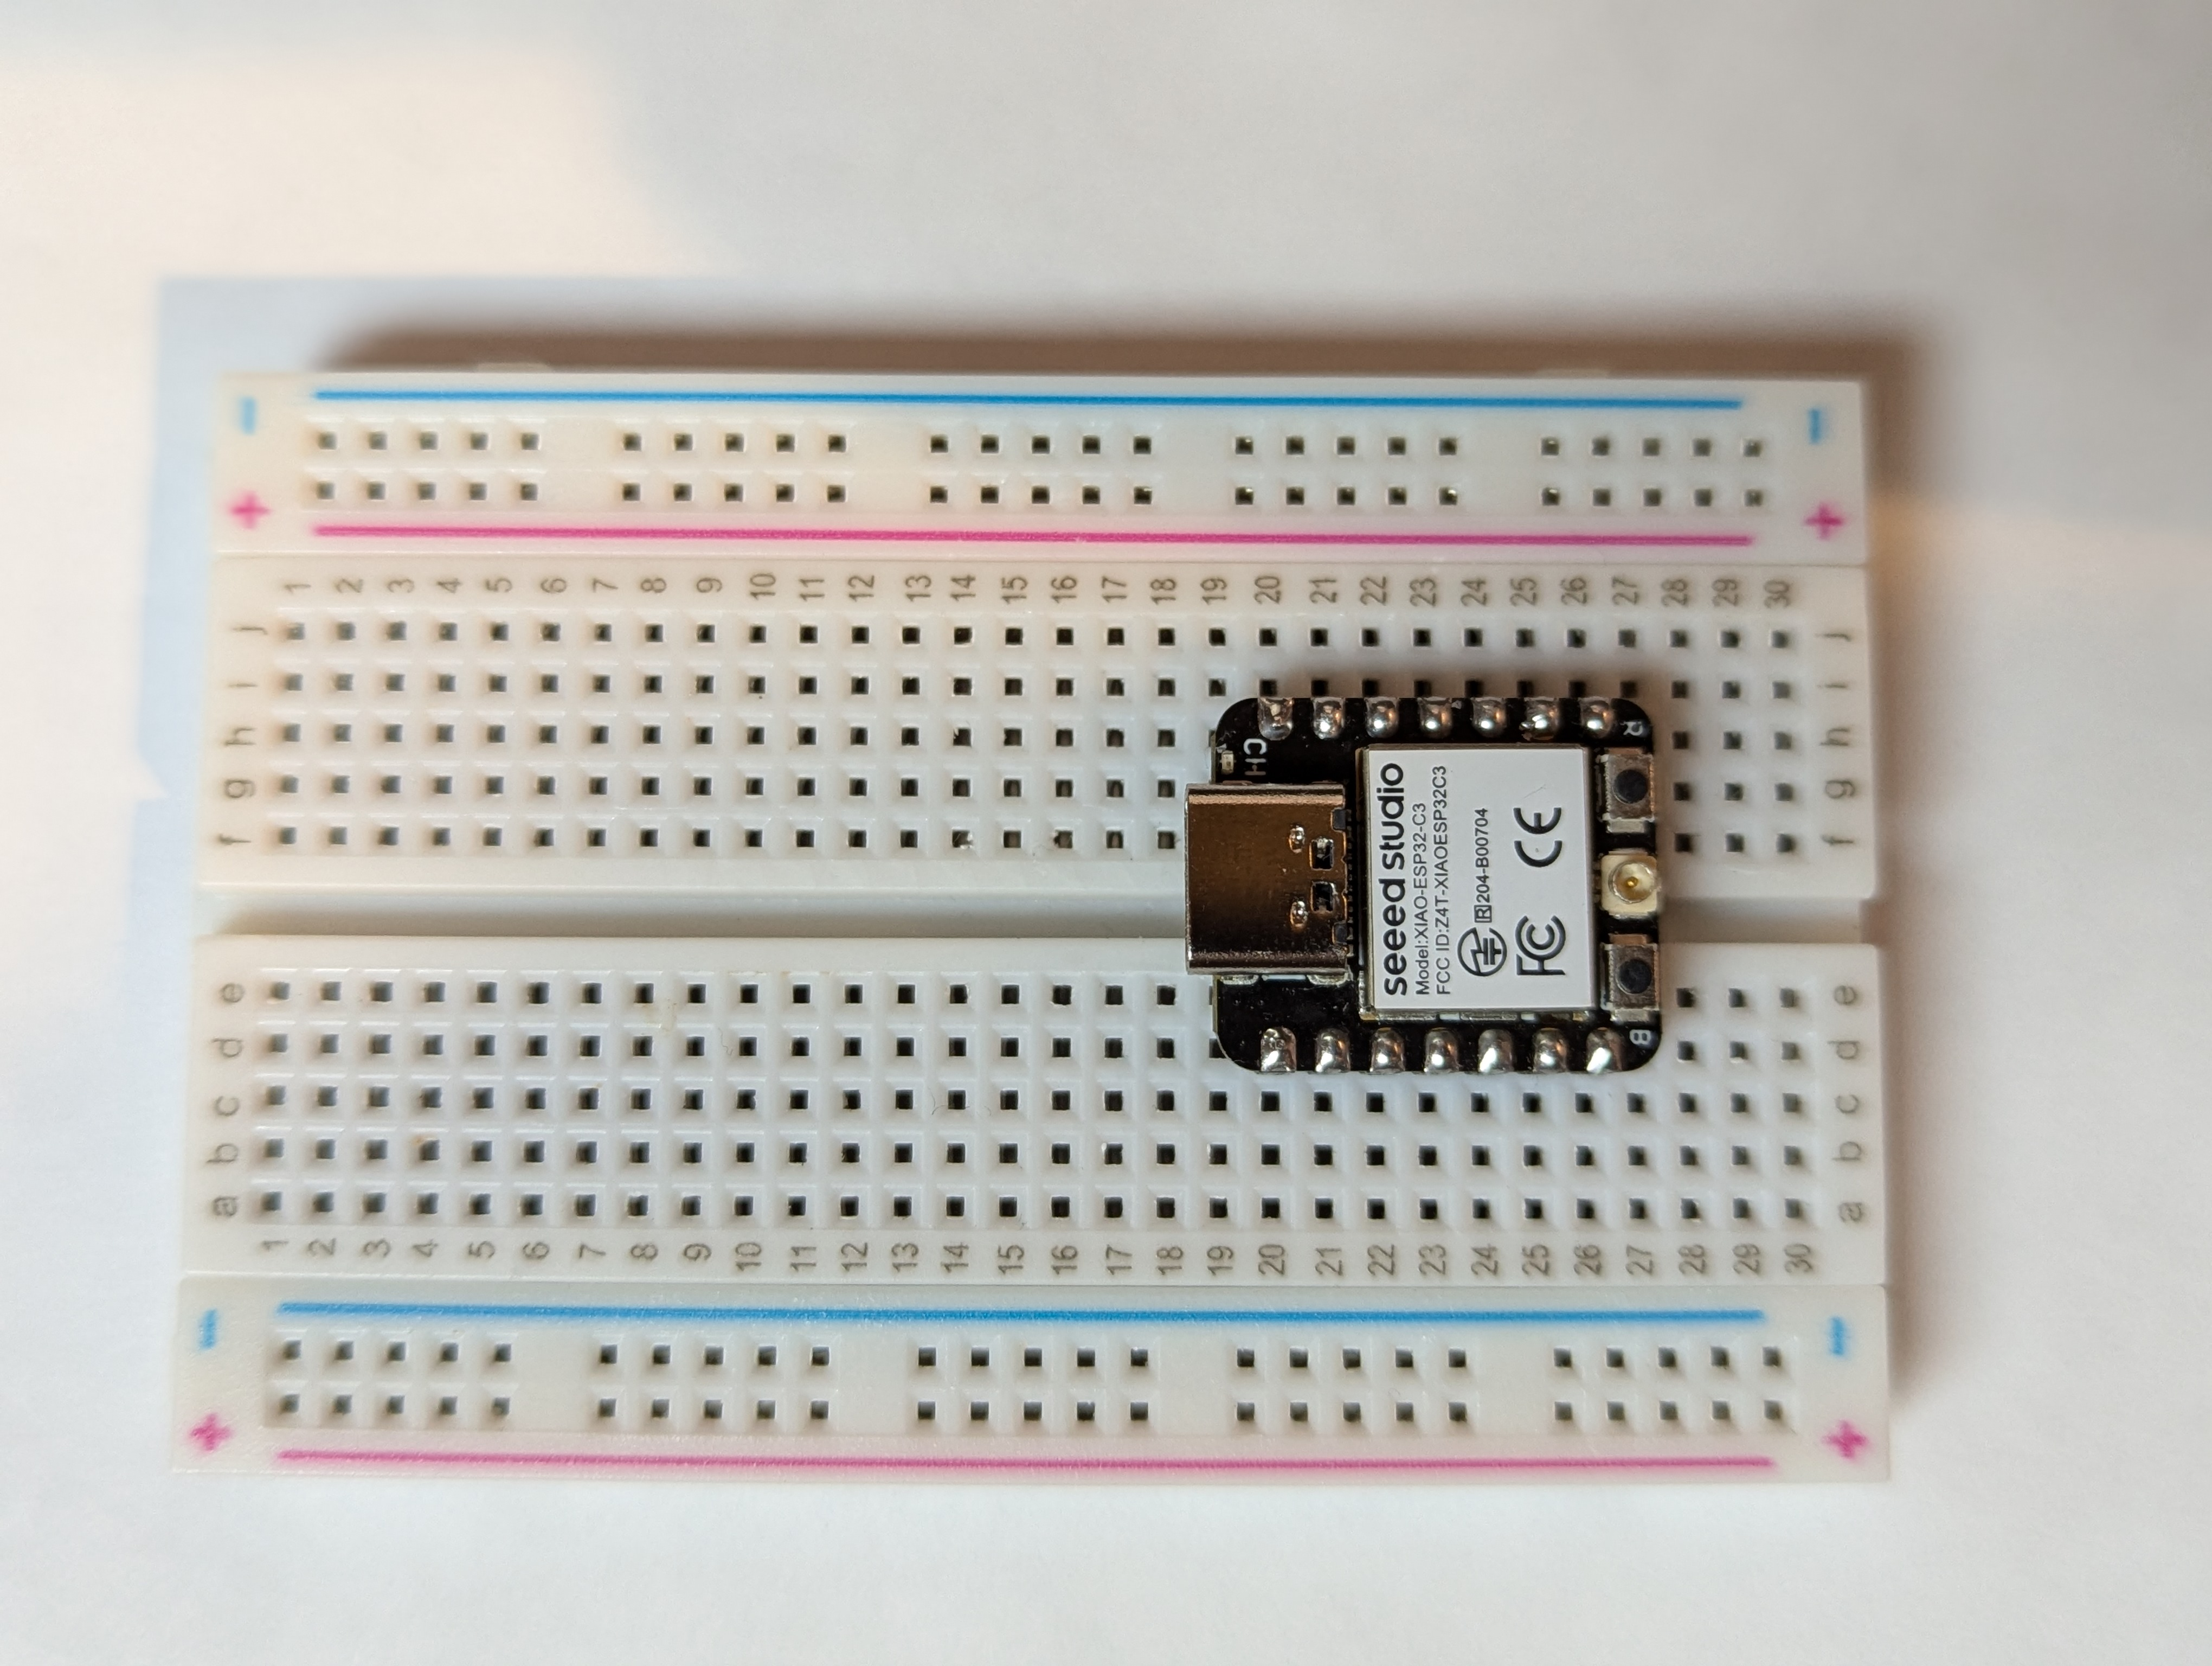
\includegraphics[width=.6\linewidth]{common/microcontroller_seated_in_breadboard.jpg}
    \caption{So far, so good!}
\end{figure}

\subsubsection{Connect the LED, Button, and Resistors}
\begin{itemize}
    \item Place a red LED into the breadboard with the longer leg in \textbf{C11} and the shorter leg
    in \textbf{C12}. Then place one leg of a resistor in \textbf{A12} and the other in the bottom
    negative rail (the blue one).
    \item Place a red LED into the breadboard with the longer leg in \textbf{C14} and the shorter leg
    in \textbf{C15}. Then place one leg of a resistor in \textbf{A15} and the other in the bottom
    negative rail.
    \item Place a red LED into the breadboard with the longer leg in \textbf{C17} and the shorter leg
    in \textbf{C18}. Then place one leg of a resistor in \textbf{A18} and the other in the bottom
    negative rail.
    \item Place a red LED into the breadboard with the longer leg in \textbf{C20} and the shorter leg
    in \textbf{C21}. Then place one leg of a resistor in \textbf{A21} and the other in the bottom
    negative rail.
    \item Place the button so that one connected set of pins (refer to \ref{button_basics} for an example) is in \textbf{E28}
    and \textbf{F28} and the other set is in \textbf{E30} and \textbf{F30}.
    \item Finally place a resistor between \textbf{B30} and the bottom negative rail.
\end{itemize}

You should be left with something that looks like this:
\begin{figure}[H]
    \centering
    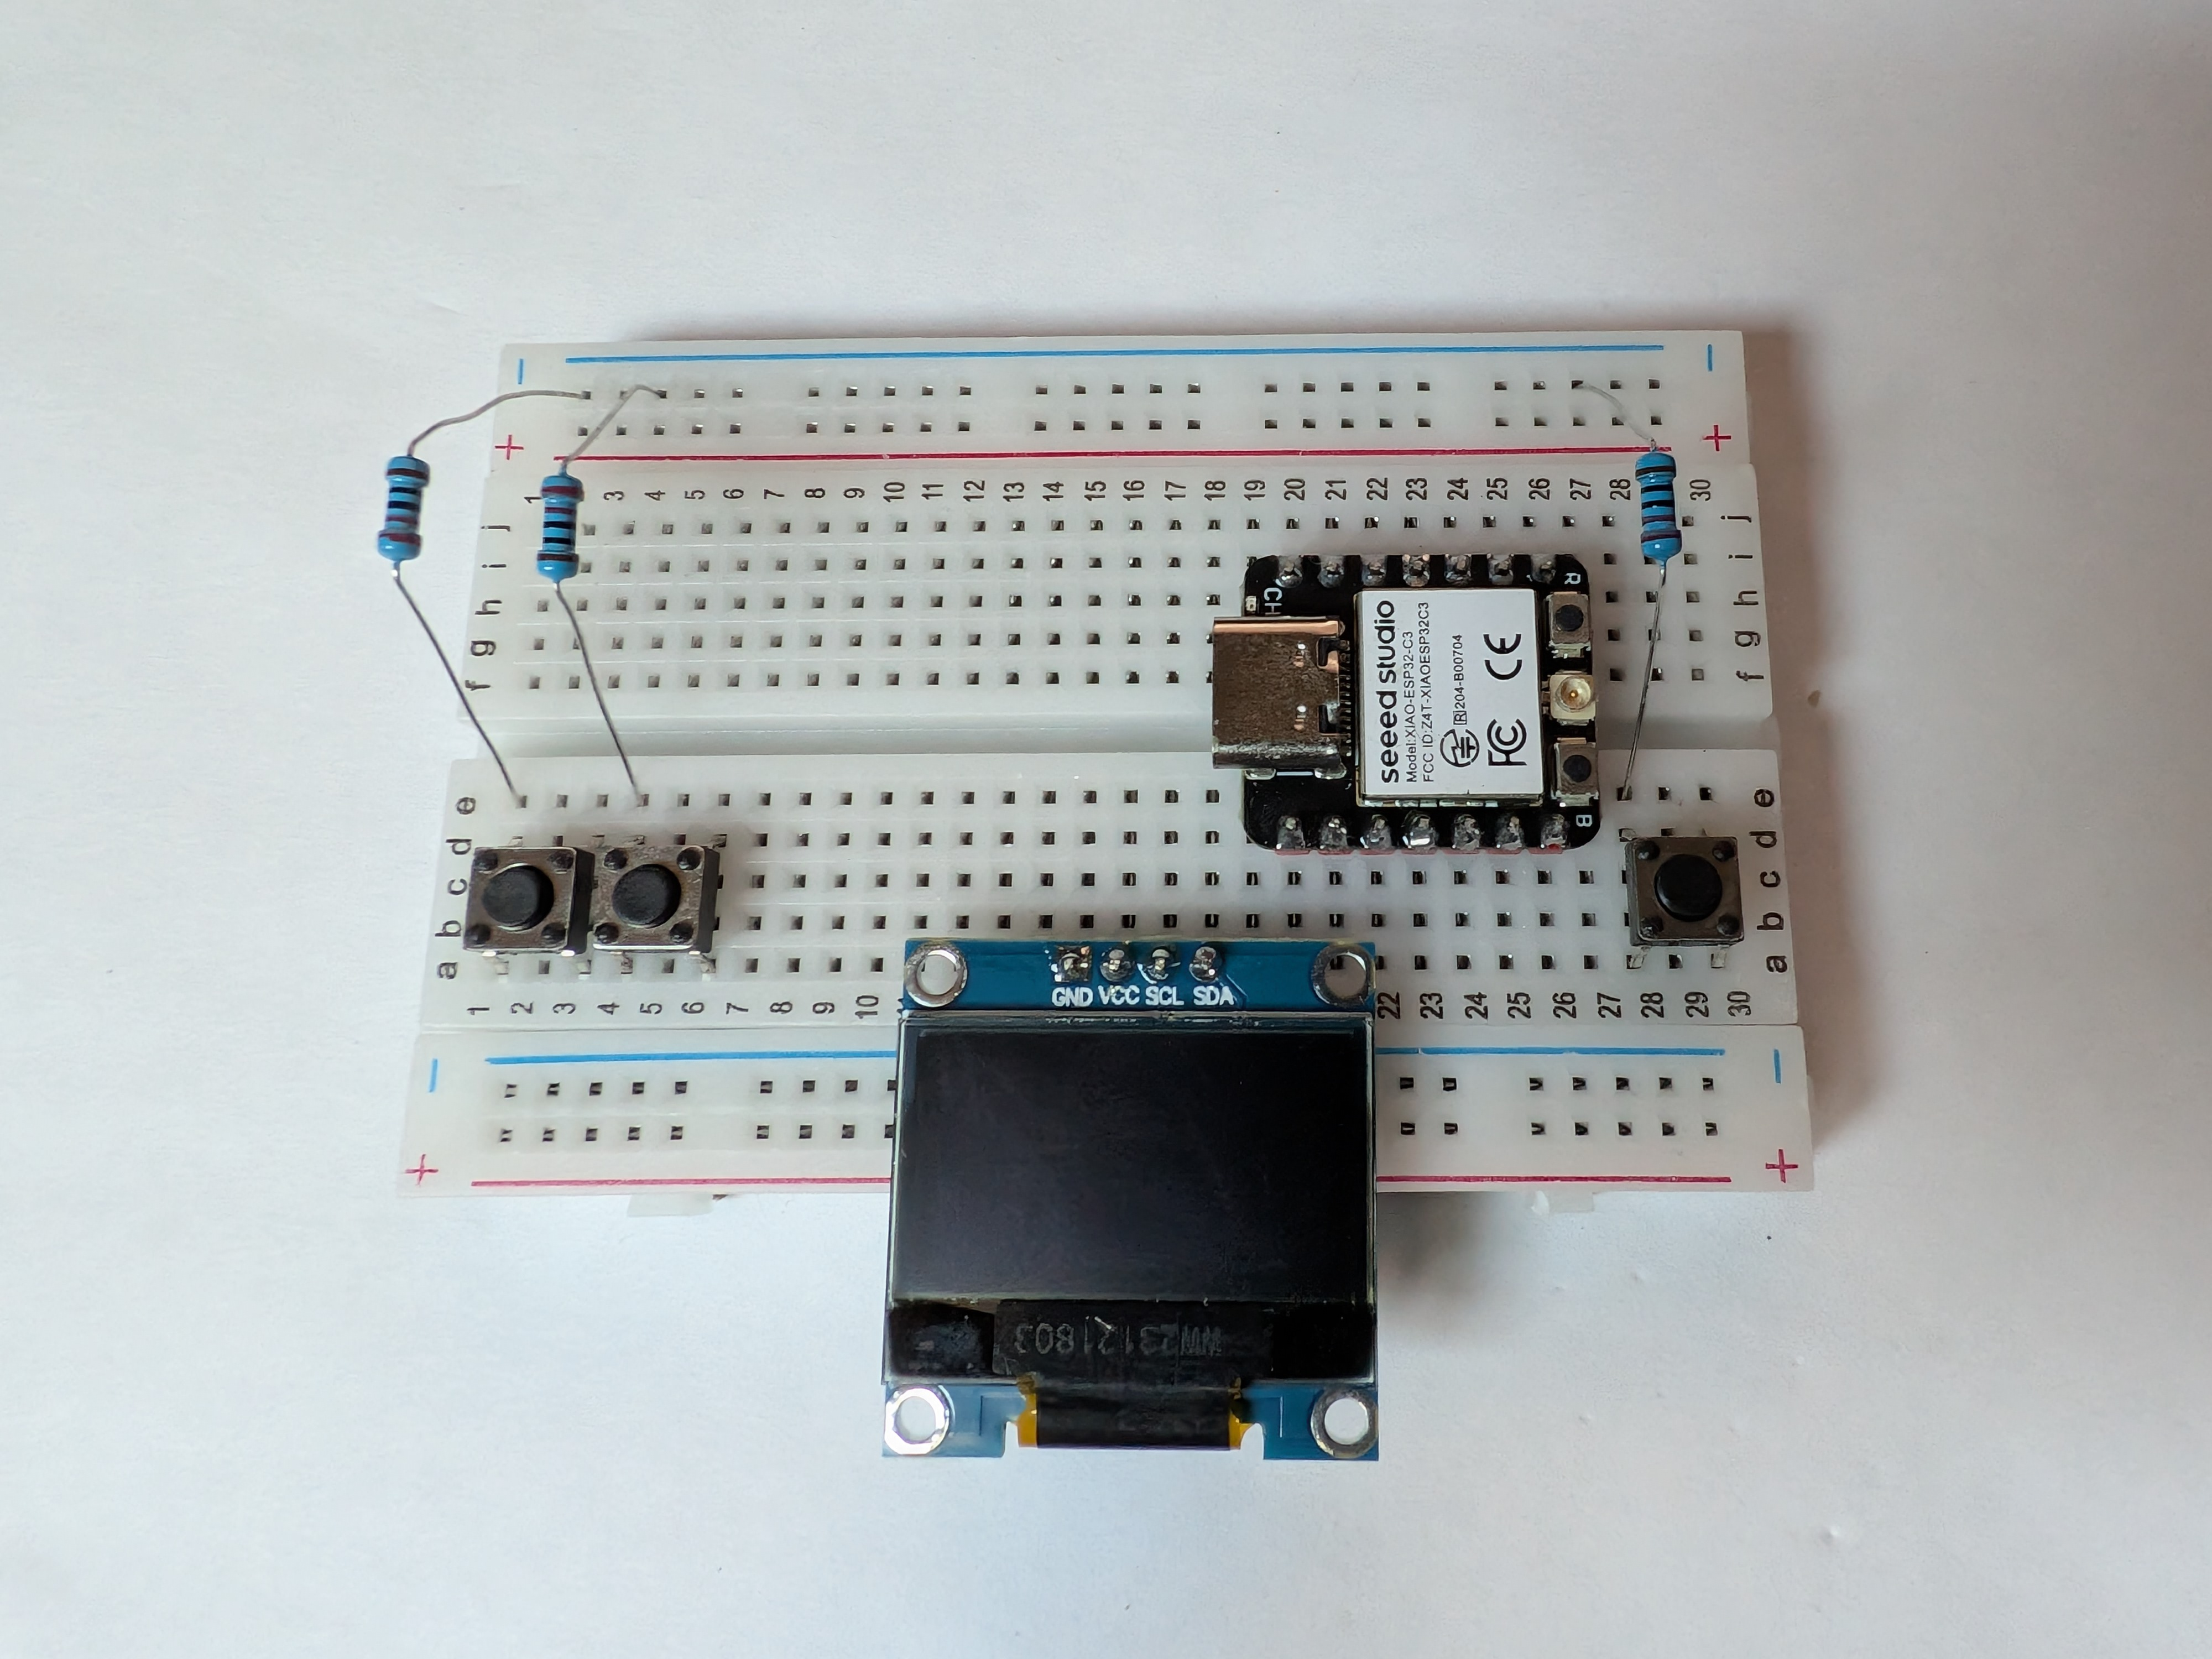
\includegraphics[width=.55\linewidth]{project_3/components_placed.jpg}
    \caption{All of the components except for the jumper wires are now placed.}
\end{figure}

\subsubsection{Connect the necessary jumper wires}
\begin{itemize}
    \item Place one end of a red jumper wire into hole \textbf{B1} of the breadboard and the other end into
    \textbf{E11}. This will provide \textbf{3.3} volts of power to the red LED when the program turns it on.
    \item Place one end of a yellow jumper wire into hole \textbf{B2} of the breadboard and the other end into
    \textbf{E14}. This will provide \textbf{3.3} volts of power to the yellow LED when the program turns it on.
    \item Place one end of a green jumper wire into hole \textbf{B3} of the breadboard and the other end into
    \textbf{E17}. This will provide \textbf{3.3} volts of power to the green LED when the program turns it on.
    \item Place one end of a purple jumper wire into hole \textbf{B4} of the breadboard and the other end into
    \textbf{E20}. This will provide \textbf{3.3} volts of power to the blue LED when the program turns it on.
    \item Using a black jumper wire, place one end of the wire into hole \textbf{J2} of the breadboard and the other
    end into the bottom negative rail (the blue one). This will provide a ground path for all of the components
    in the circuit.
    \item Place a white jumper wire into hole \textbf{J7} and the other end into \textbf{J28}. This will
    provide the signal to the microcontroller when the button is pushed.
\end{itemize}

You should be left with something that looks like this:
\begin{figure}[H]
    \centering
    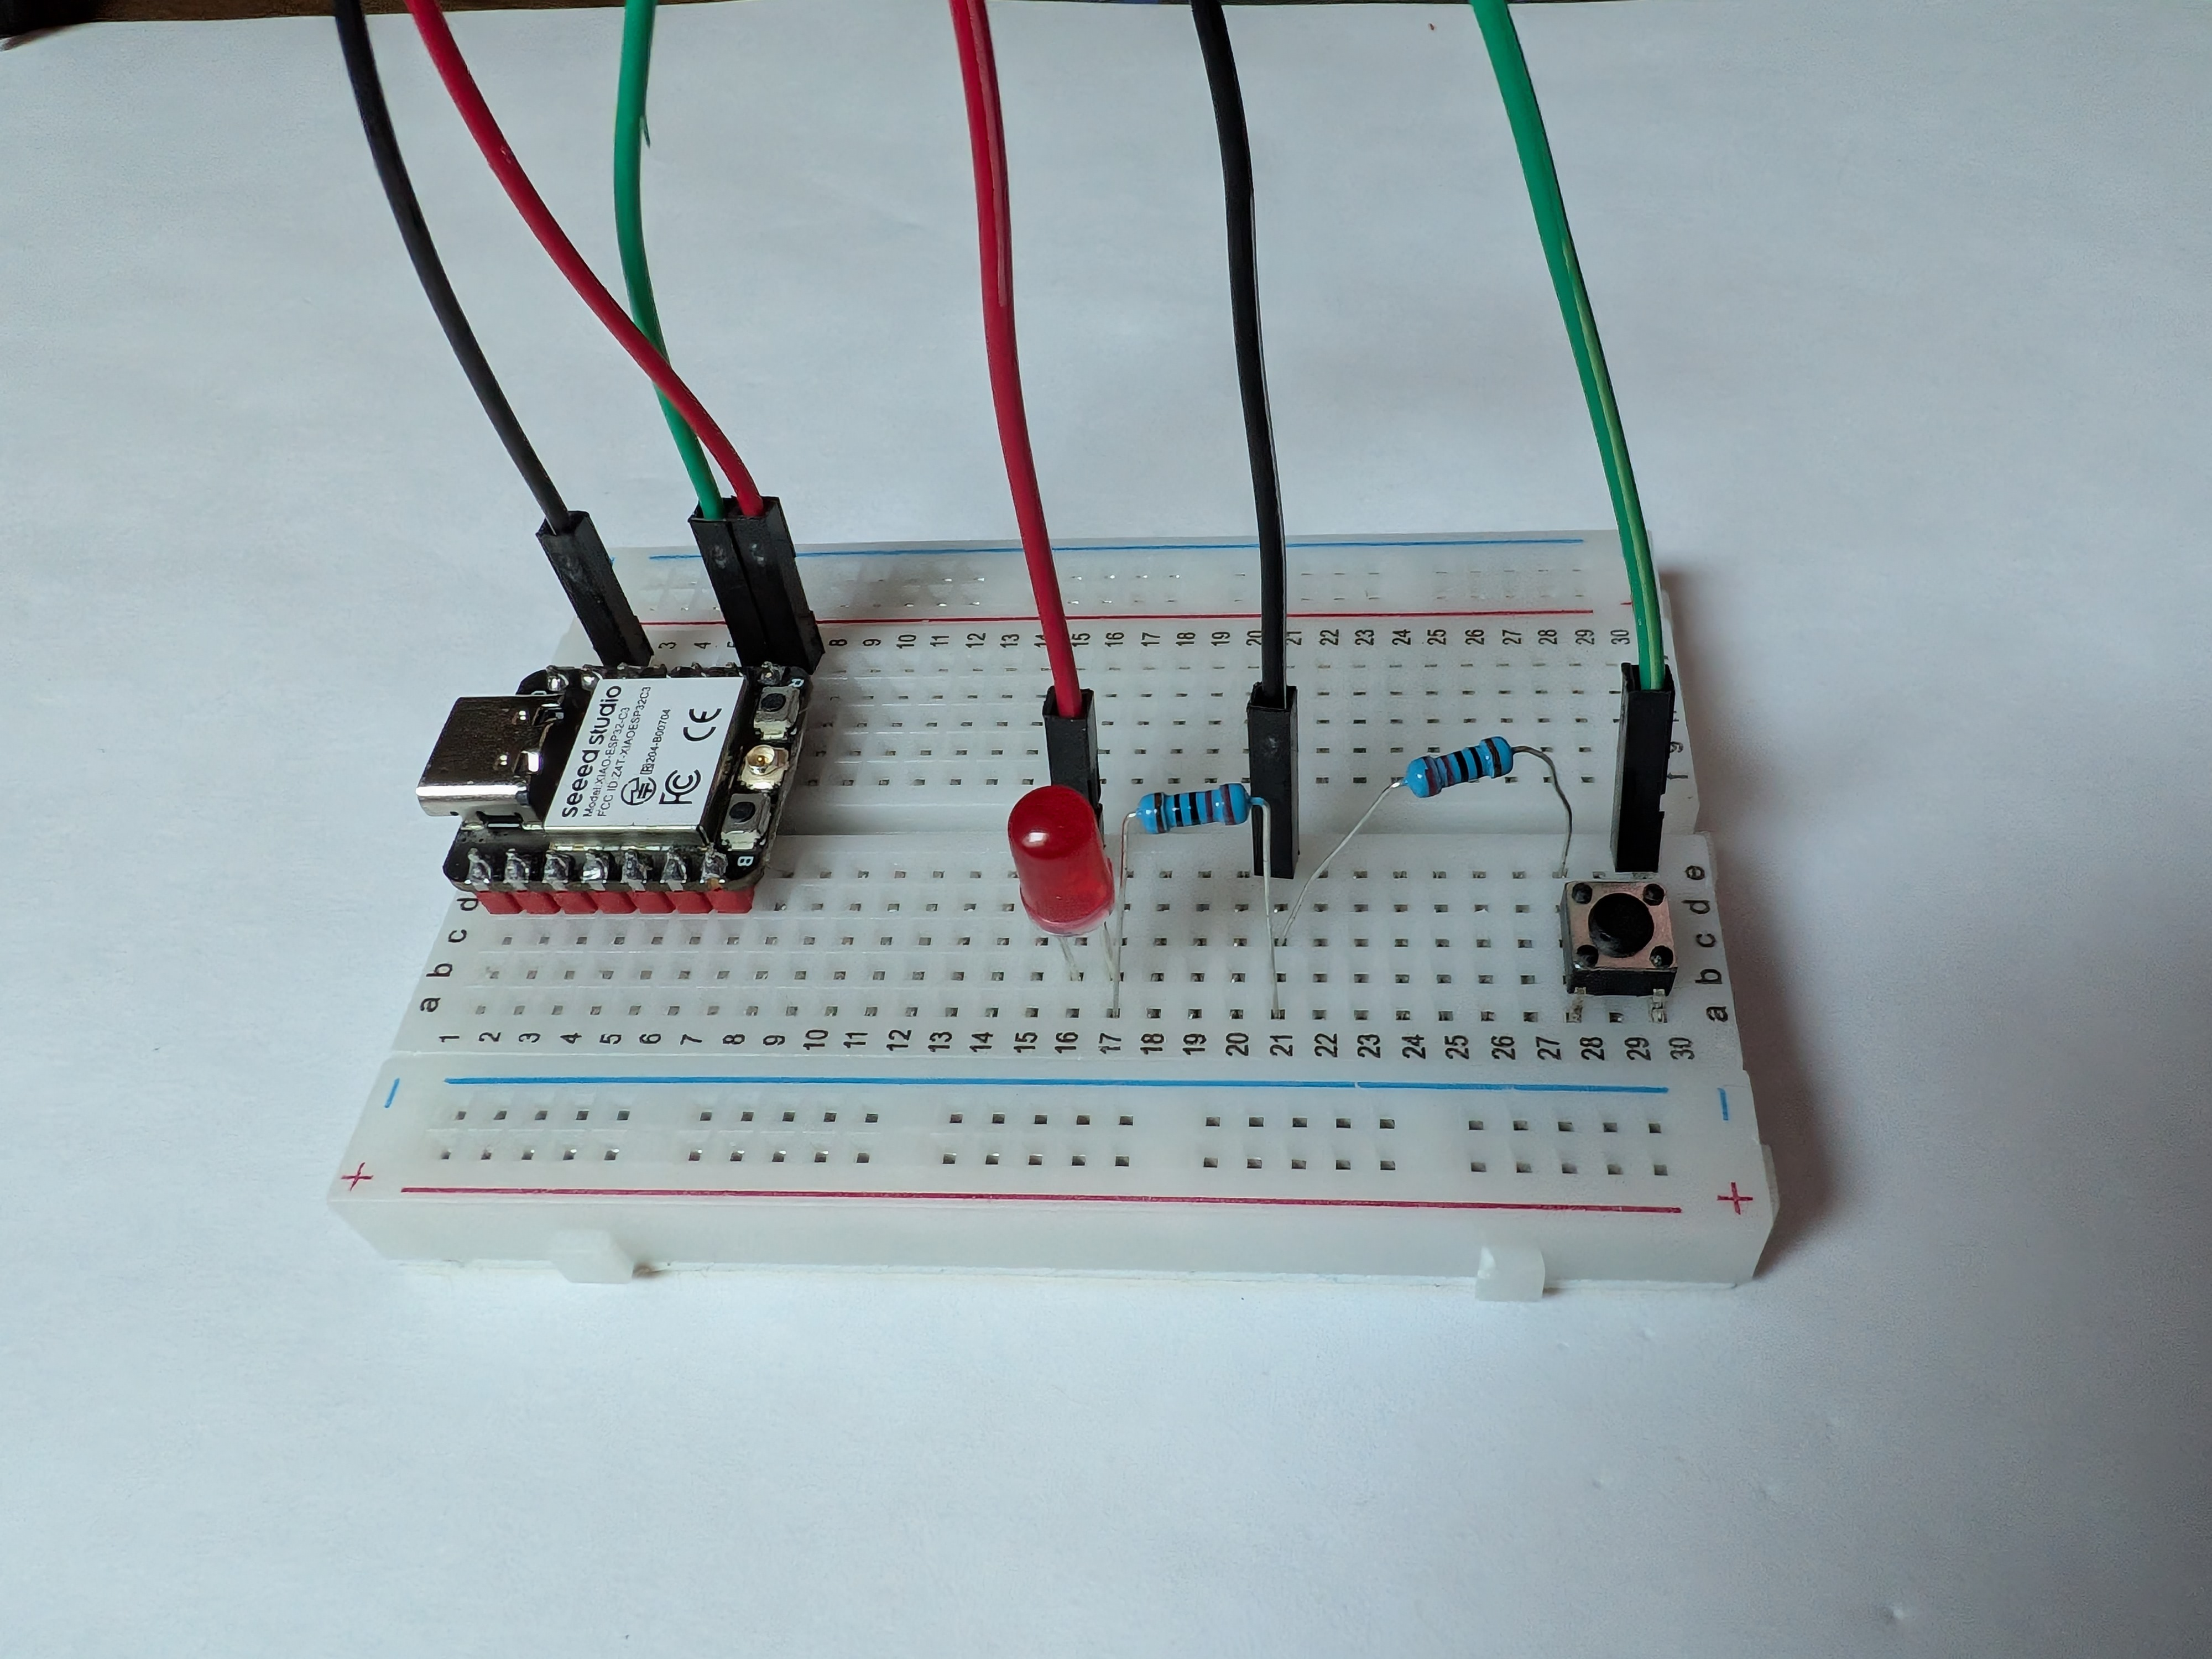
\includegraphics[width=.55\linewidth]{project_3/all_wired_up.jpg}
    \caption{All of the components except for the jumper wires are now placed.}
\end{figure}

\subsection{Programming the microcontroller}

Once all of the wiring is correct, connect the USB cable to the microcontroller and load the IDE to
access it. Refer back to Chapter \ref{ide} for instructions.

Click on the file named "project\_3\_led\_party.py". This will load the code in the editor for this section.
Read through the comments and the code to get a sense for how it works. Once you are ready, you can
click the blue play button in the upper left of the window to start the script.

While the script is running, the LEDs will animate with one of 5 pre-programmed animations. Pressing
the button will cycle to the next animation.

\section{Review}
In this project, we learned how we can add interactivity to a circuit by using momentary pushbuttons.
These buttons can be read from the microcontroller's code to run a piece of code (called an interrupt)
whenever they are pressed.

\section{Possible Extensions}
If you want to do some experimentation, try these:

\begin{itemize}
    \item Add different animation functions that you come up with and add them to the cycle
    \item Add a second button and have it control the brightness of the LEDs at the same time that
    the first button controls the pattern (hint: you'll need to always set them in PWM mode)
\end{itemize}
